\documentclass{beamer}
\beamertemplatenavigationsymbolsempty
\graphicspath {{../images/}}

\usepackage{amsmath}
\newcommand{\bra}[1]{\langle#1\rvert} % Bra
\newcommand{\ket}[1]{\lvert#1\rangle} % Ket
\newcommand{\qprod}[2]{ \langle #1 | #2 \rangle} %Inner Product
\newcommand{\braopket}[3]{\langle #1 | #2 | #3\rangle} % Matrix Element
\newcommand{\expect}[1]{ \langle #1 \rangle} % Expectation value
\newcommand\abs[1]{\left|#1\right|}

% Theme
\usetheme{Boadilla}

% Title page
\title{Optimalizácia variačných kvantových eigensolverov}
\author{Michal Švec}
\institute{doc. RNDr. Martin Plesch, PhD.}
\date{December 6, 2023}

\makeatother
\setbeamertemplate{footline}
{
  \leavevmode%
  \hbox{%
  \begin{beamercolorbox}[wd=.3\paperwidth,ht=2.25ex,dp=1ex,center]{author in head/foot}%
    \usebeamerfont{author in head/foot}\insertshortauthor
  \end{beamercolorbox}%
  \begin{beamercolorbox}[wd=.6\paperwidth,ht=2.25ex,dp=1ex,center]{title in head/foot}%
    \usebeamerfont{title in head/foot}\insertshorttitle
  \end{beamercolorbox}%
  \begin{beamercolorbox}[wd=.1\paperwidth,ht=2.25ex,dp=1ex,center]{date in head/foot}%
    \insertframenumber{} /\inserttotalframenumber\hspace*{1ex}
  \end{beamercolorbox}}%
  \vskip0pt%
}
\makeatletter
\setbeamertemplate{navigation symbols}{}
\setbeamertemplate{itemize items}[circle]
\setbeamertemplate{caption}{\raggedright\insertcaption\par}



% Begin document
\begin{document}

% Title slide
\begin{frame}
	\titlepage
\end{frame}

\begin{frame}
	\frametitle{Kvantové počítače}
		
	\begin{columns}[c]
		\begin{column}{.6\textwidth}
			\centering
						      
			\begin{itemize}
				\item 0K = = -273.15°C
				      
			\end{itemize}
		\end{column}
				      
		\begin{column}{.4\textwidth}
			\centering
						          
			\begin{figure}
				\centering
				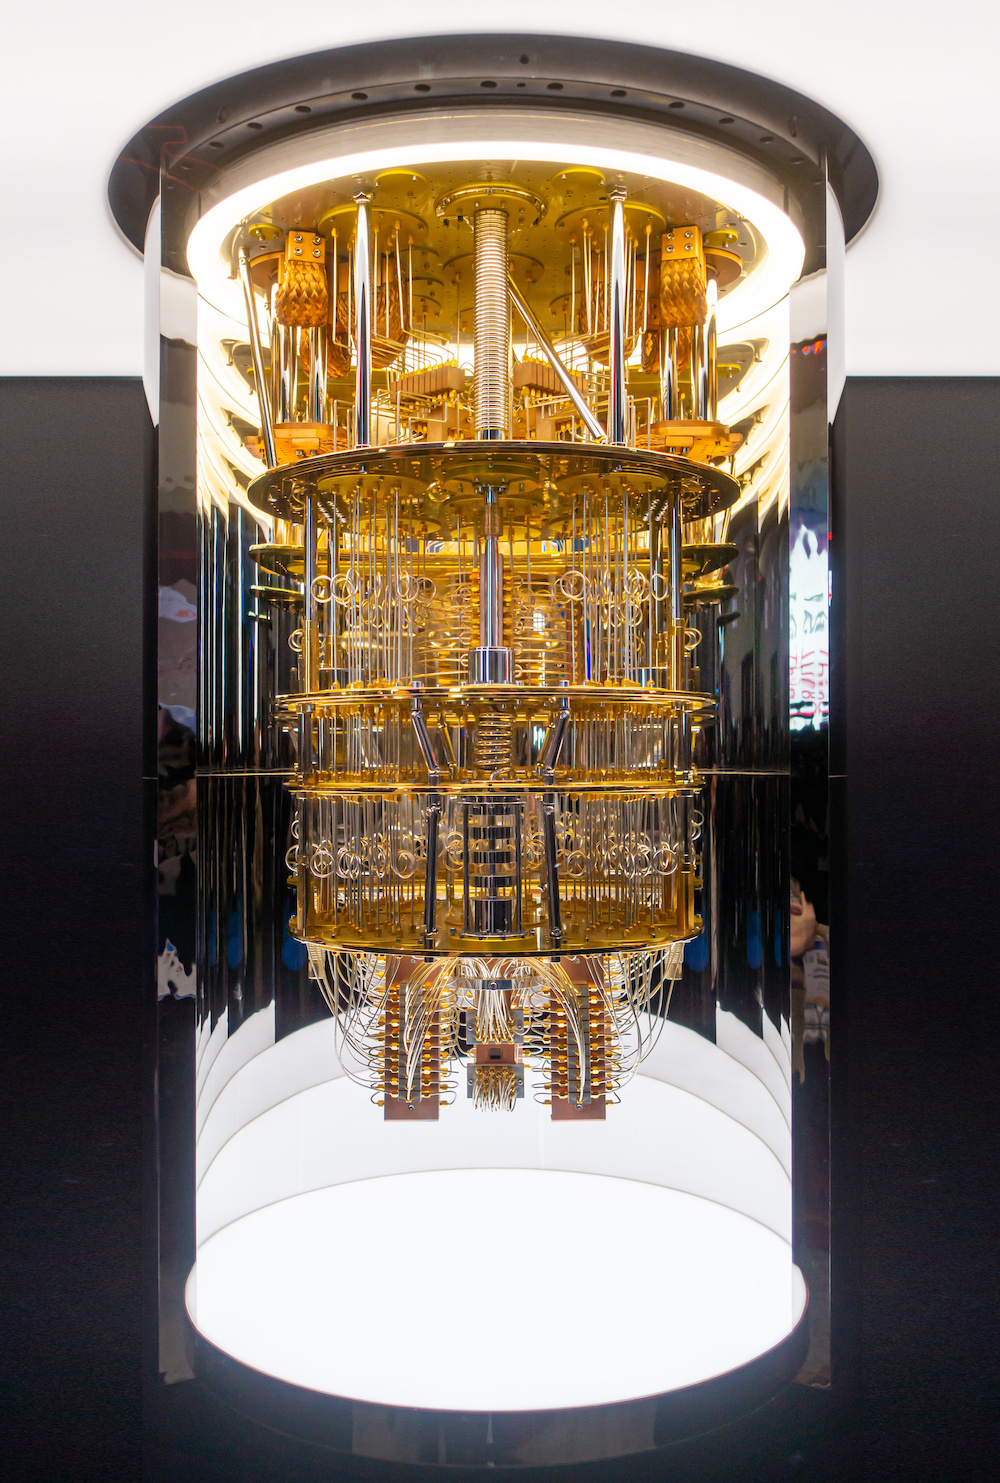
\includegraphics[width=1\textwidth]{quantum_computer.jpeg}            
			\end{figure}
		\end{column}
	\end{columns}
		
		
		
\end{frame}

\begin{frame}
	\frametitle{Bit vs Qubit}
	\begin{columns}[t]
		\begin{column}{.5\textwidth}
			\centering
			Bit (\textbf{b}inary dig\textbf{it})  
			\vspace{0.4cm} 
			\begin{itemize}
				\centering
				\item najmenšia jednotka informácie v štandardnom počítači
				\item booleovská algebra
				      
			\end{itemize}
		\end{column}
				      
		\begin{column}{.5\textwidth}
			\centering
			Qubit (quantum bit)
			\vspace{0.4cm}
			\begin{itemize}
				\centering
				\item najmenšia jednotka informácie v kvantovom počítači
				\item lineárna algebra nad Hilbertovým priestorom

			\end{itemize}		
		\end{column}
	\end{columns}
	% \begin{figure}
	% 	\centering
	% 	\includegraphics[width=0.3\textwidth]{bit_vs_qubit.jpg}            
	% \end{figure}
\end{frame}

\begin{frame}
	\frametitle{Reprezentácia qubitov}
	\begin{itemize}
		\item matice
		\item block sphere {\color{red} TODO ako sa to preklada?}
		\item $\ket{\psi} = \begin{pmatrix}
		      \alpha \\
		      \beta
		\end{pmatrix}$, kde $\abs{\alpha}^2 + \abs{\beta}^2 = 1$ 
	\end{itemize}
	\begin{columns}[c]
		\begin{column}{.3\textwidth}
			\centering
			$\ket{0} = \begin{pmatrix}
			1\\
			0
			\end{pmatrix}$
			\begin{figure}
				\centering
				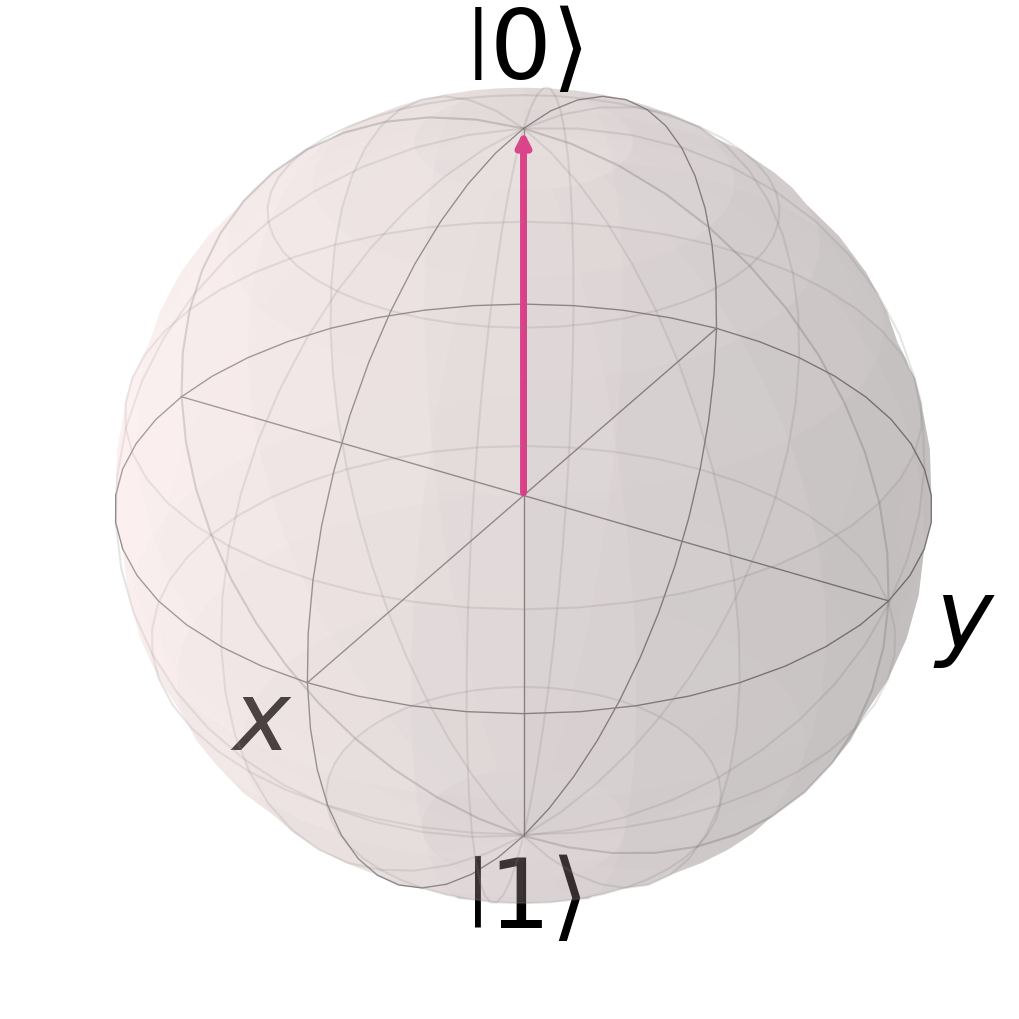
\includegraphics[width=1\textwidth]{qubit0.png}            
			\end{figure}
		\end{column}
				
		\begin{column}{.3\textwidth}
			\centering
			$\ket{1} = \begin{pmatrix}
			0\\
			1
			\end{pmatrix}$
			\begin{figure}
				\centering
				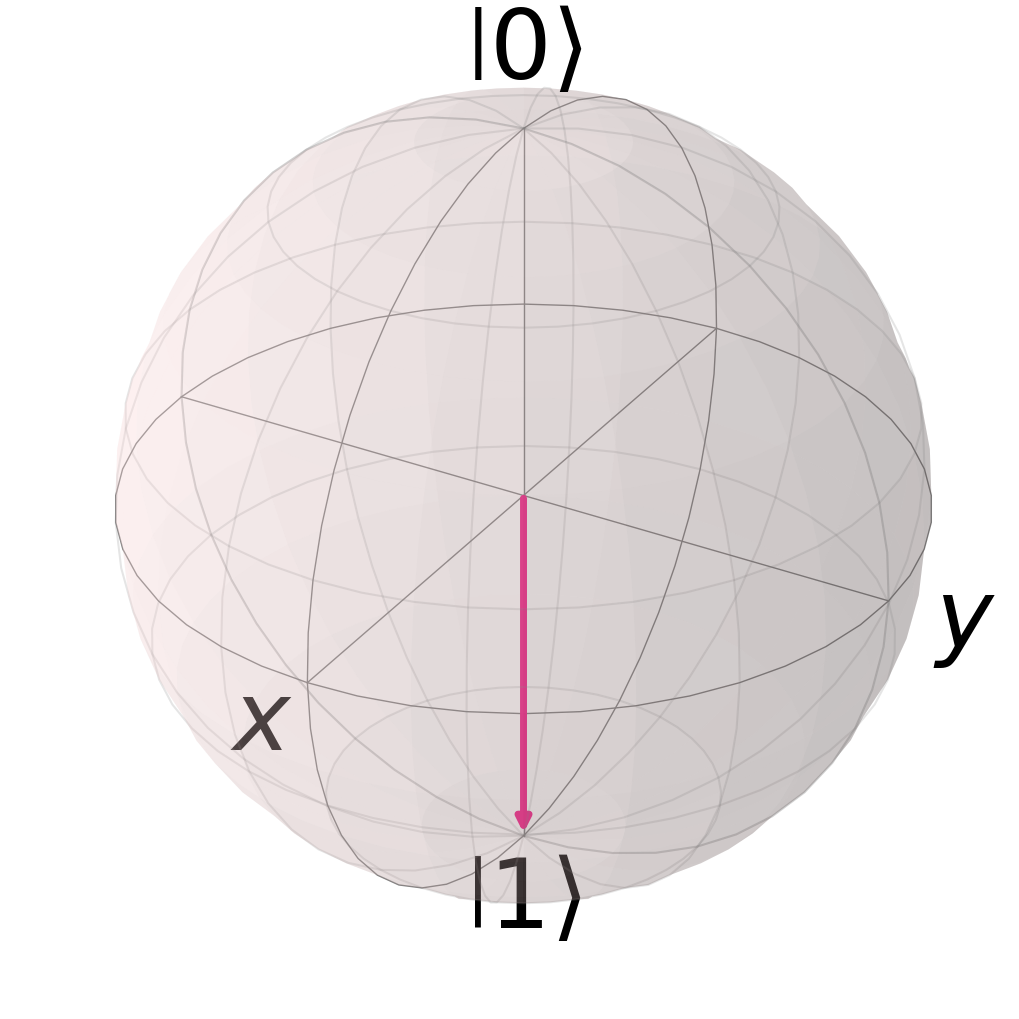
\includegraphics[width=1\textwidth]{qubit1.png}            
			\end{figure}
		\end{column}
				
		\begin{column}{.3\textwidth}
			\centering
			$H\ket{0} = \begin{pmatrix}
			\frac{1}{\sqrt{2}}\\
			\frac{1}{\sqrt{2}}
			\end{pmatrix}$
			\begin{figure}
				\centering
				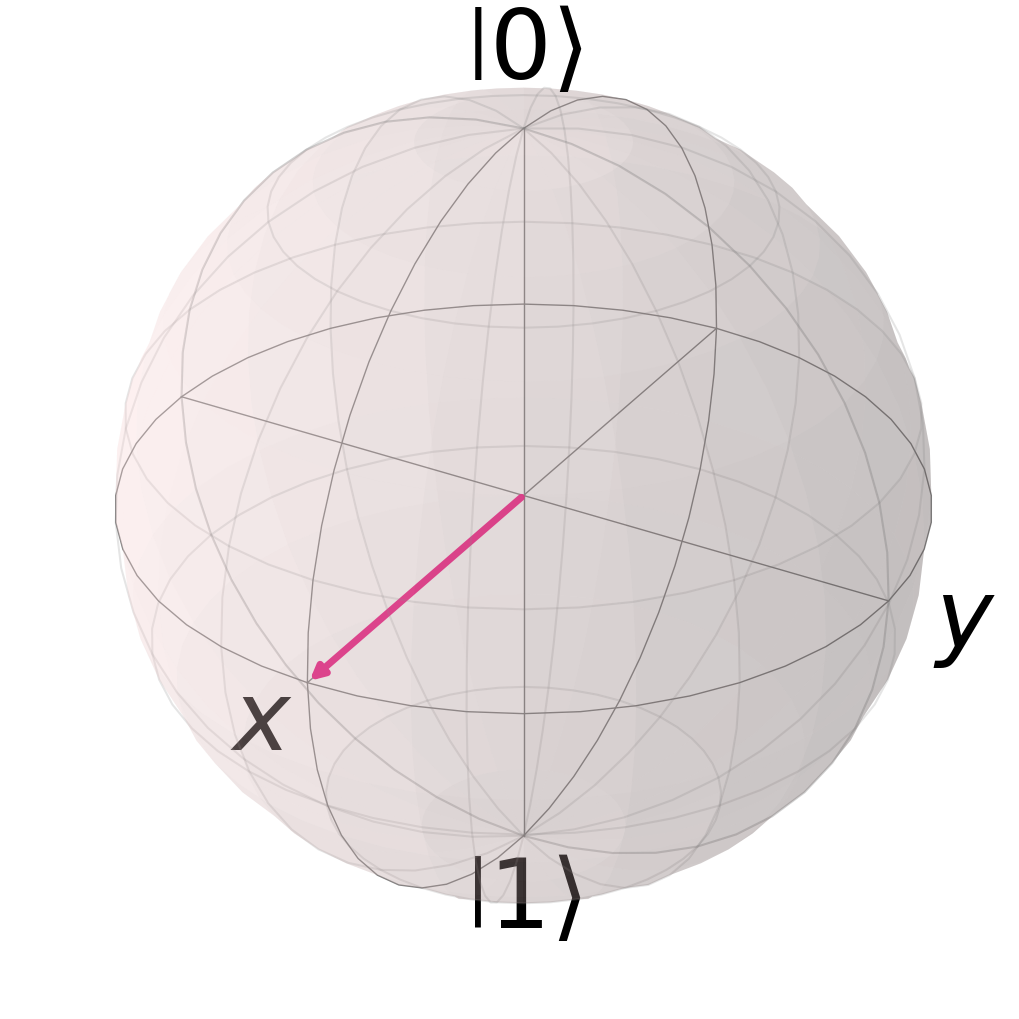
\includegraphics[width=1\textwidth]{qubith.png}            
			\end{figure}
		\end{column}
	\end{columns}
		    
\end{frame}

\begin{frame}
	\frametitle{Operácie na bitoch a qubitoch}
	\begin{columns}[t]
		\begin{column}{.5\textwidth}
			\centering
			% first column about standard gates
			Logické hradlá
			\vspace{0.4cm}
			\begin{itemize}
				\item NOT
			\end{itemize}
			     
			\begin{columns}[c]
				% NOT gate image
				\begin{column}{.5\textwidth}
					\begin{figure}
						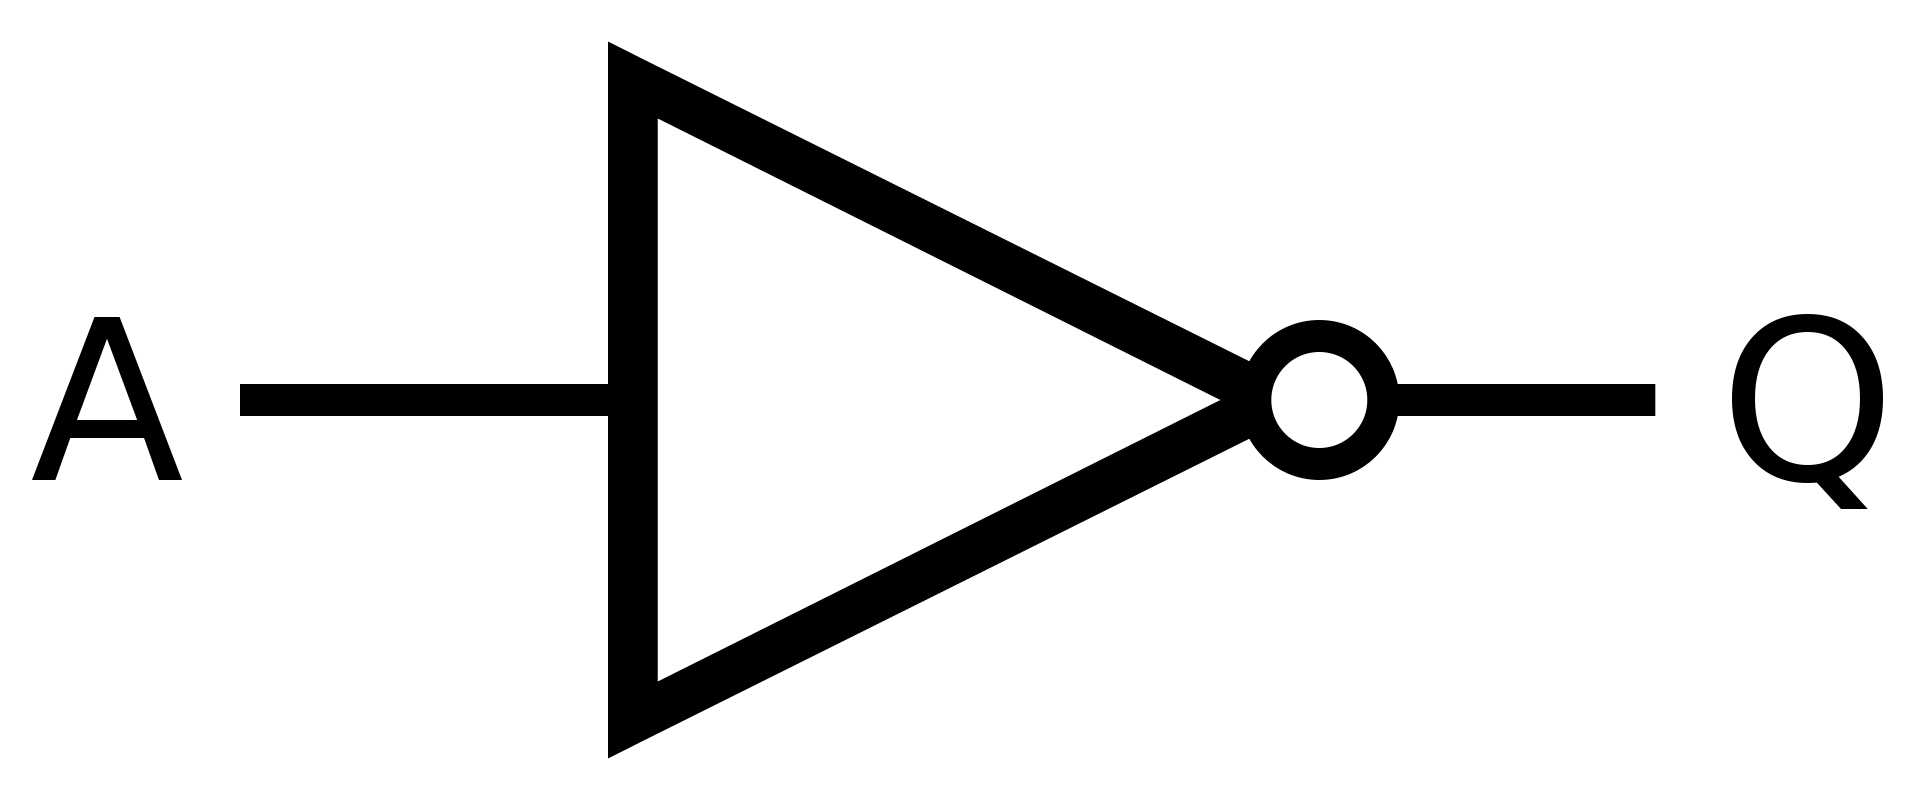
\includegraphics[width=.5\textwidth]{standard_not_gate.png}            
					\end{figure}
				\end{column}
				% NOT gate table
				\begin{column}{.5\textwidth}
					\begin{displaymath}
						\begin{array}{|c|c|}
							\hline
							A & Q \\
							\hline
							0 & 1 \\
							\hline
							1 & 0 \\
							\hline
						\end{array}   
					\end{displaymath}    
				\end{column}
			\end{columns}
			\begin{itemize}
				\item AND
			\end{itemize}
			\begin{columns}[c]
				\begin{column}{.5\textwidth}
					\begin{figure}
						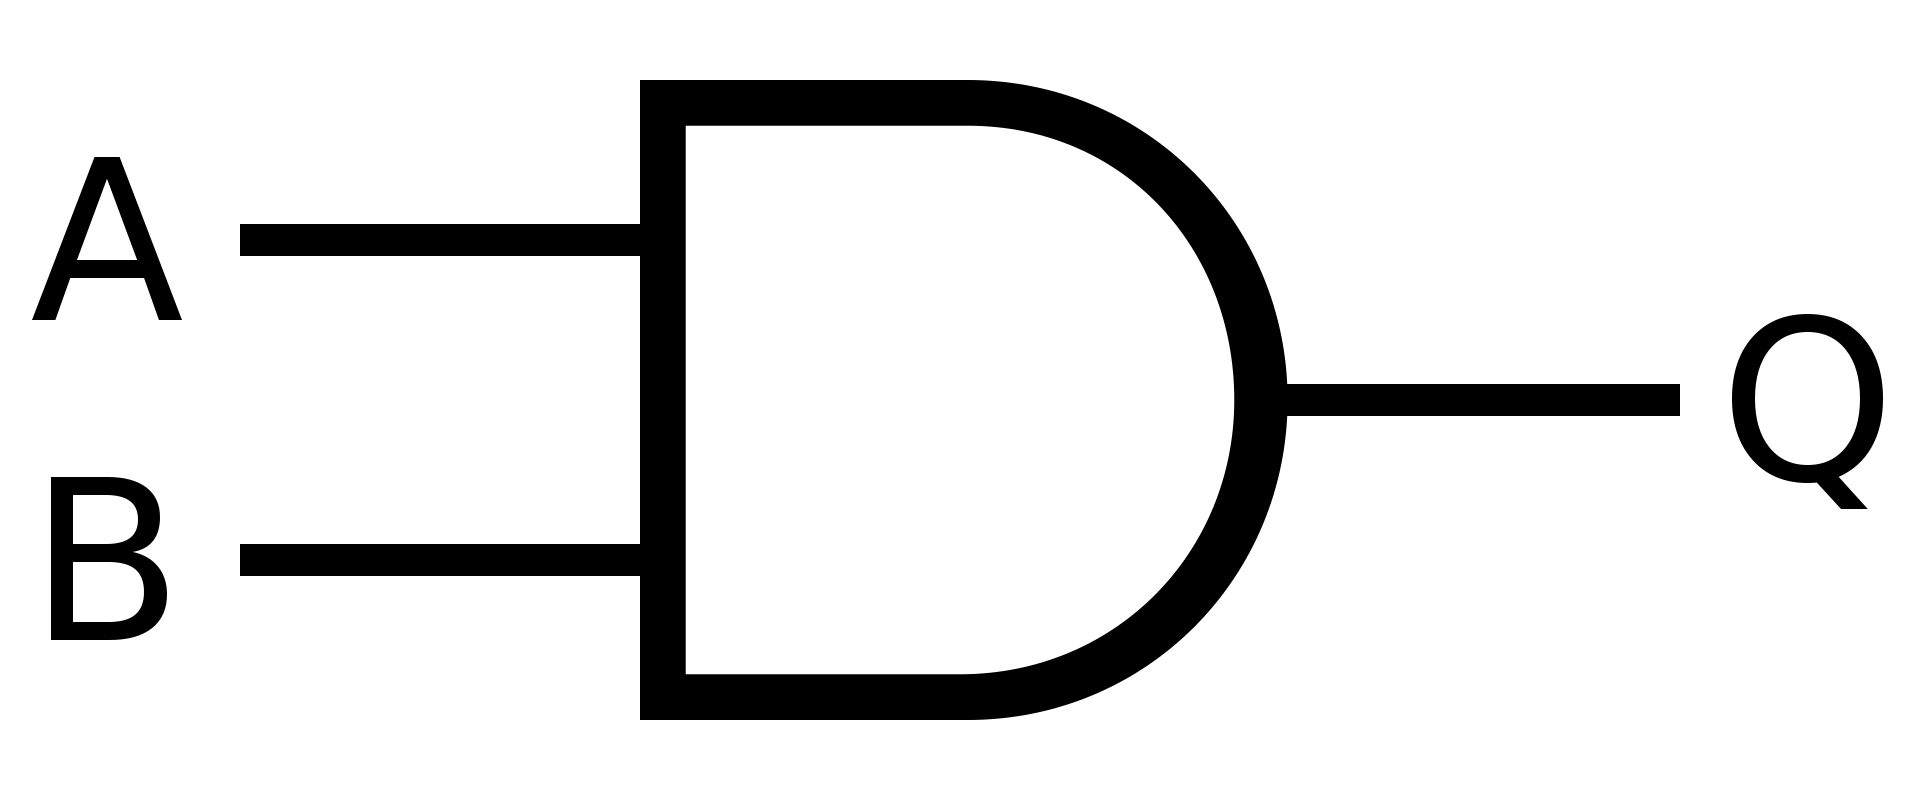
\includegraphics[width=.5\textwidth]{standard_and_gate.png}            
					\end{figure}
				\end{column}
				\begin{column}{.5\textwidth}
					\begin{displaymath}
						\begin{array}{|c c|c|}
							\hline
							A & B & Q \\ 
							\hline 
							0 & 0 & 0 \\
							\hline
							1 & 0 & 0 \\
							\hline
							0 & 1 & 0 \\
							\hline
							1 & 1 & 1 \\
							\hline
						\end{array}   
					\end{displaymath}
				\end{column}
			\end{columns}
			\begin{itemize}
				\item ...
			\end{itemize}
			
		\end{column}
		
		% second column about standard gates
		\begin{column}{.5\textwidth}
			\centering
			Kvantové hradlá
			\vspace{0.4cm}
			\begin{itemize}
				\item Hadamard
			\end{itemize}
					
			\begin{columns}[c]
				% first gate image
				\begin{column}{.5\textwidth}
					\begin{figure}
						\centering
						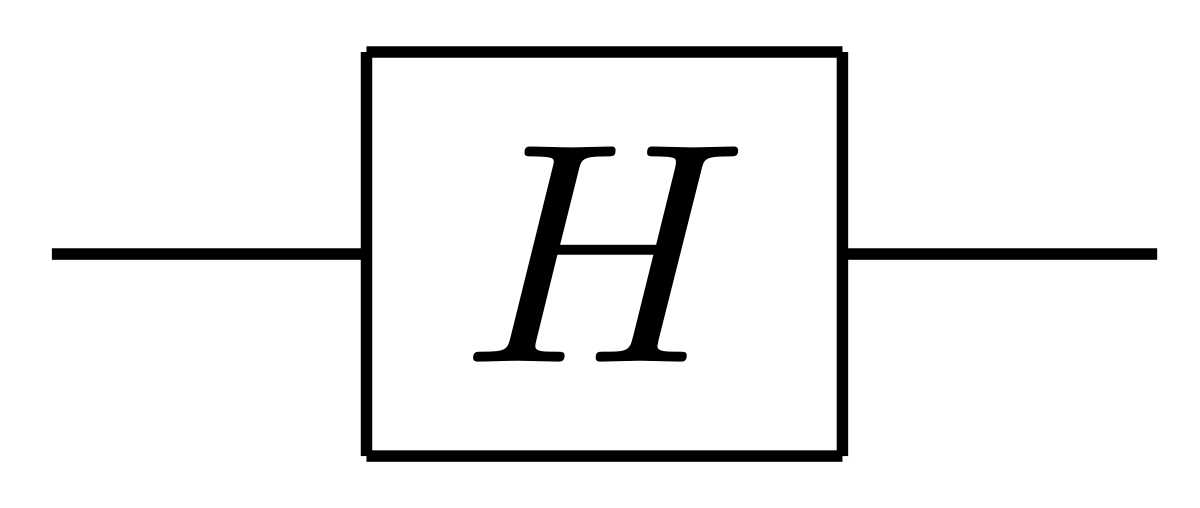
\includegraphics[width=0.5\textwidth]{hadamard_gate.png}
					\end{figure}
				\end{column}
				
				% hadamard gate matrix
				\begin{column}{.5\textwidth}
					$\frac{1}{\sqrt{2}}\begin{pmatrix}
					1 & 1\\
					1 & -1\\
					\end{pmatrix}$
				\end{column}
			\end{columns}  
			\begin{itemize}
				\item       Control NOT
				      
			\end{itemize}
				
				
			\begin{columns}[c]
								
				\begin{column}{.5\textwidth}
					% CNOT gate image
					\begin{figure}
						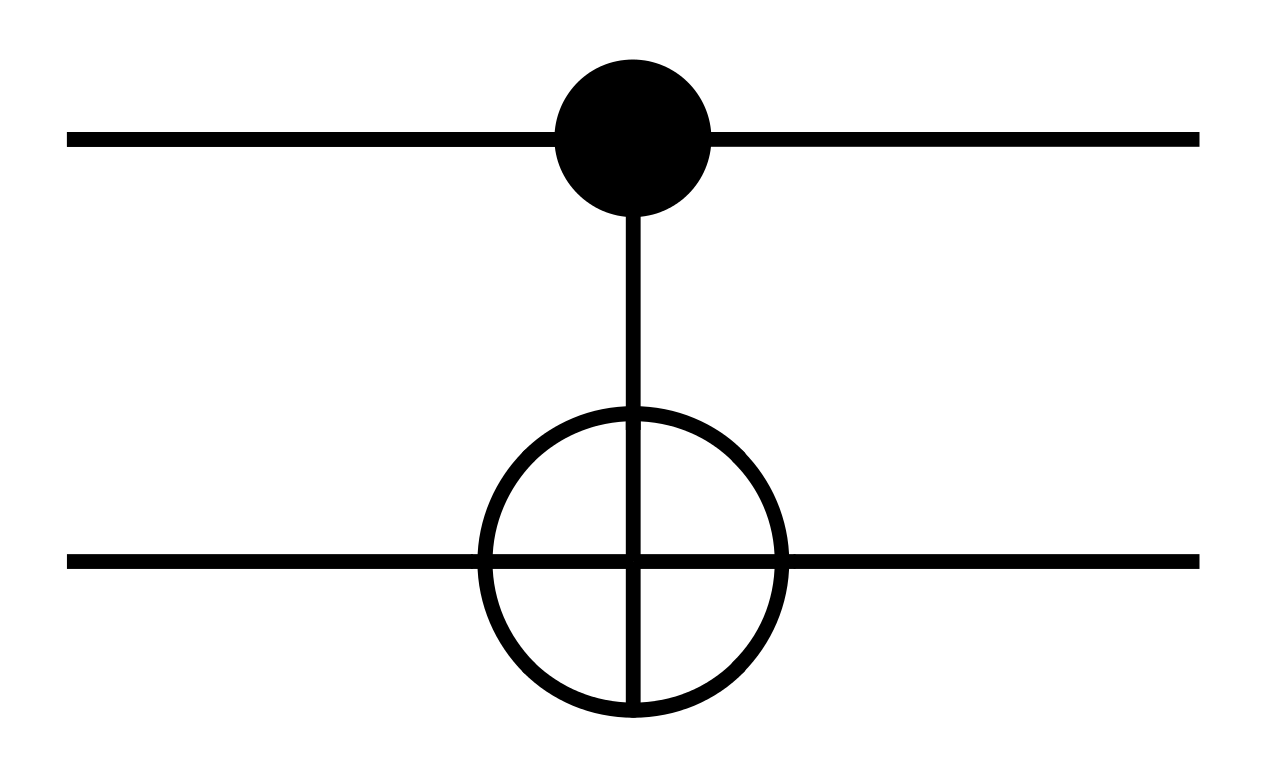
\includegraphics[width=0.5\textwidth]{cnot_gate.png}
					\end{figure}
				\end{column}
				% CNOT gate matrix
				\begin{column}{.5\textwidth}
					$\frac{1}{\sqrt{2}}\begin{pmatrix}
					1 & 0 & 0 & 0\\
					0 & 1 & 0 & 0\\
					0 & 0 & 0 & 1\\
					0 & 0 & 1 & 0\\
					\end{pmatrix}$
				\end{column}
					
			\end{columns}
			\begin{itemize}
				\item ...
				      
			\end{itemize}
		\end{column}
	\end{columns}     
	        
		
		  
\end{frame}

\begin{frame}
	\frametitle{Superpozícia \& kvantové previazanie}
	Superpozícia
	\begin{itemize}
		\item $\ket{\psi} = \alpha\ket{0} + \beta\ket{1}$
		\item $\abs{\alpha}^2 + \abs{\beta}^2 = 1$
		
	\end{itemize}
	Kvantové previazanie
	\begin{itemize}
		\item $\ket{\psi} = \alpha\ket{00} + \beta\ket{11}$
		\item $\abs{\alpha}^2 + \abs{\beta}^2 = 1$
		
	\end{itemize}
\end{frame}


\begin{frame}
	\frametitle{Variačný kvantový eigensolver (VQE)}
	\begin{itemize}
		\item hybridný algoritmus
		      \begin {itemize}
		\item klasický počítač
		\item kvantový počítač 
	\end{itemize}
	\item variačný princíp
	\item eigensolver
	\end{itemize}
		
	\begin{figure}
		\centering
		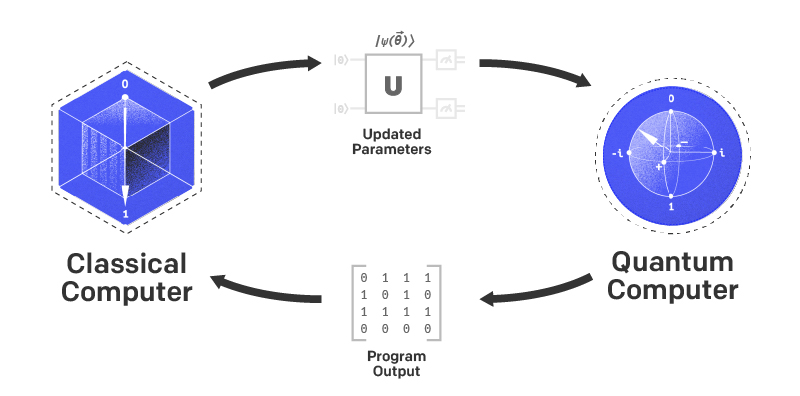
\includegraphics[width=0.75\textwidth]{vqe.jpeg}
		\caption{VQE}
				            
	\end{figure}
\end{frame}


\begin{frame}
	\frametitle{Ciele bakalárskej práce}
	\begin{itemize}
		\item budeme používať knižnicu Qiskit
		\item TODO obrazok kvantoveho obvodu z qiskitu
		      \begin{itemize}
		      	\item open source Python knižnica vyvíjaná IBM
		      	\item nepoužívame skutočný kvantový počítač, používame simulátor
		      	\item TODO meranie collapsses
		      	\item TODO vstup a vystup, su to matice?
		      	\item \begin{figure}
		      	      \centering
		      	      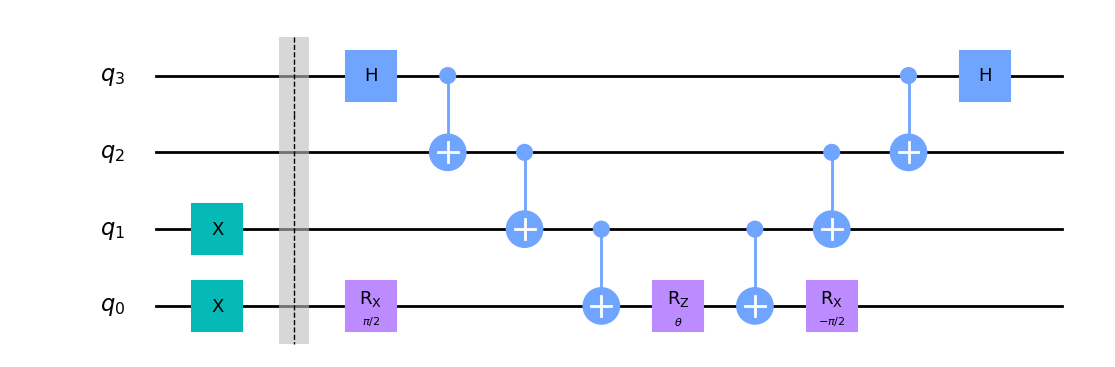
\includegraphics[width=0.75\textwidth]{quantum_circuit.png}
		      	\end{figure}
		      \end{itemize}
		      		            
	\end{itemize}
\end{frame}
\end{document}